\section{Flow of Events}
\label{sec:flow_of_events}

The lifecycle of a piece of collateral, and its UTXO Set on-chain, can be broadly split into two stages (refer to Figure \ref{fig:architecture-diagram}):

\begin{enumerate}
    \item \textbf{Minting}. This is the initiation of the UTXO set. The Wallet software creates the smart contract by using the CDM type system, and consumes an existing UTXO representing the balance of the party minting the collateral to create two new UTXOs: the contract and the remaining balance.  
    \item \textbf{Posting/Updates}. At regular time intervals the state of the UTXO Set is updated to reflect changes in collateral valuation (note that this functionality is not currently implemented but could easily be achieved by running a \textit{"cron job"} \footnote{A "cron job" process is a scheduled task or automated script in Unix-like operating systems that runs at specified intervals without the need for manual initiation \citep{cronjobs}.} process in the background). The updating transactions consumes two inputs, the current contract state and balance of the counterparty, and produces two new UTXOs: the updated contract state (potentially containing a different amount of satoshis) and the updated balance. These updates can be of two types:
    
    \begin{enumerate}
        \item \textbf{Posting/Receiving Collateral}. This type of update refers to movement of satoshi to either the contract or the party's balance depending of the new valuation.
        
        \item \textbf{Updating Contract Terms}. this type of update allows the custodian to modify the business logic of the contract (e.g. the eligibility of an existing or new type of collateral could be updated). Recounting that legal and economic terms from both the ISDA Master Agreement and the CSAs can be updated in the current sysytem, supporting this functionality is core to a smooth transition the on-chain solution.
    \end{enumerate}
    
    In the current implementation 3pm New York Time (ET) has been arbitrarily chosen as the time to update the UTXO Set, however this level of granularity is quite rough and would not account for intra-day valuation variations. An additional piece of functionality that constantly monitors the state of the market and the valuation of the collateral and updates the UTXO Set whenever a specified threshold valuation is passed would be a good solution to reflect large swings in the market. This is suggested as future work on the this thesis. \label{ny3pm}
\end{enumerate}

A more granular view of the flow of events is provided in Figure \ref{fig:sequence-diagram}, where a sequence diagram of the system is described. The two sections of the sequence diagram correspond to the Minting and Updating stages described above.

\begin{enumerate}
    \item \textbf{Minting}. Let us assume that a custodian is in charge of interacting with the chain. The act of minting requires three smart contracts to be written, the Relationship, the Portfolio and the Position (details on the contents of each are described in more detail in Section \ref{sec:mapping}). The custodian will first deploy the Relationship contract. Only after this has been deployed on-chain can the custodian include the address of its UTXO in the Portfolio contract and deploy the latter. A key aspect of mechanism of the current system is that all objects (within the collateral context as well as beyond it) contain references to each other, and such interconnectedness allows for easy retrieval and inspection beginning with any starting point (one could go back to the trading relationship between parties from a specific collateral position or vice versa, fetch all the positions contained within a relationship). Adapting this mechanism on-chain involves reflecting any change to a '\textit{sub-contract}' (hereby defined as a contract referenced by another one) by updating the \textit{'parent'} contract(s) (the referencing contracts). In the Minting scenario just described, the fact that the Portfolio contract has been deployed must be propagated upwards to the corresponding Relationship within which the Portfolio is contained. In a similar manner, when the Portfolio has been deployed, the Position contracted can be filled in with the Portfolio UTXO's address, published on chain and the deployment information (which takes the form of a UTXO address itself) propagated up the stack to the Portfolio and the Relationship. \label{minting}
    
    \item \textbf{Updating}. The type of update described here corresponds to the movements of satoshis following a change in collateral valuation. Updates of the legal and/or economic terms have not been implemented as the core value proposition of this work is to streamline the valuation and margin-posting elements. While contract term updates would be a required feature of a fully CDM-compliant system, we leave this implementation as future work. Margin calculation and posting follow the steps desribed below:

    \begin{enumerate}
    
        \item \label{item:legal_econ_terms} The Wallet must compute the Mark-to-Market (MTM) valuation for the asset. Depending on specific type of asset, the MTM calculation may vary (e.g. for commodities this is simply the spot price multiplied by the quantity of the asset held as collateral, while for interest rate swaps more detailed calculations involving the fixed and floating rates, as well as the market rates for the corresponding fixed and floating rates, are required). For the purpose of a proof-of-concept, this thesis uses a commodity, crude oil, as collateral. Note that the system is easily extendable to support other types of commodities simply by plugging in the MTM valuation models that a counterparty may already use. The commodity spot price is fetched from the party's preferred traditional financial API, e.g. the Bloomberg terminal. This work used the free and open-source Yahoo Finance library \citep{yfinance, yfinance_python} (see Appendix \ref{app:oracles_yfinance}. In the initial version of the system we planned to use an oracle to provide the spot price and/or MTM, since relying on a traditional API introduces the risk of valuation mismatches should the parties use different sources for their calculations. We were unable to find public oracles providing the service and we attribute this to the low level of maturity of the technical ecosystem, however adapting to changes in 3rd party services provided in this context is suggested as a direction of future work.

        \item \label{item:valuation} The valuation of the collateral should be expressed in satoshis in order to facilitate the movement of collateral. Denominating the asset in satoshis require converting the preferred fiat currency of the parties to satoshis, and this could be accomplished by fetching the exchange rate from an oracle service. In this thesis we use the WitnessOnChain oracle service \citep{woc_oracle} to fetch the exchange rate between USDC and BSV (see Appendix \ref{app:oracles_yfinance}. USDC is a stablecoin, i.e. a digital token whose value is pegged to USD, in the case of USDC specifically via reserve-based pegging. Each USDC is redeemable for one dollar, and is backed by one dollar or a dollar-denominated asset with equivalent value held in accounts at regulated U.S. financial institutions. Those accounts are audited by U.S. accounting firm Grant Thornton LLP, which issues monthly attestations on the reserves backing USDC \citep{pegging_usdc}. While we initially wanted to convert from USD to BSV (as USD is the currency most widely adopted in current collateral relationships), we were not able to find an oracle service providing this specific conversion rate. While relying on USDC is not optimal, the system can be considered safe as long as the stablecoin maintains its peg. An extra layer of security to protect against the fluctuations in the USDC-BSV exchange rate would be to apply an additional haircut to the CSA of the collateral agreement, effectively treating the conversion as a traditional foreign exchange rate. A haircut is a reduction applied to the value of an asset expressed as a percentage of its value \citep{haircut}. For example, if the average fluctuation of the USDC-BSV exchange rate over the previous week was 5\%, a 5\% discount haircut could be applied to the collateral. The full implications and implementation of this solution are left as future work on this dissertation.

        \item The Wallet then fetches the current collateral value stored in the Position contract. This is required to determine whether the collateral has increased or decreased in value.

        \item \label{item:risk_calc}The Wallet then computes the new value of the collateral by using the MTM valuation and the USDC-BSV exchange rate. Note that at this stage any additional factors traditionally used in asset valuation, e.g. specific risk models such as Value-at-Risk (VaR) \citep{VaR}, SPAN (Standard Portfolio Analysis of Risk) \citep{SPAN} or custom Monte Carlo Simulations \citep{monte_carlo}, can be incorporated. Performing these calculations off-chain introduces an additional risk factor since a counterparty must trust the results that the other party provides, fundamentally nullifying one of the core value propositions of this thesis, i.e. the transparency of the margin calculations. An ideal solution would work entirely on-chain, with the calculations, or at least the parameters used in them, publicly auditable. While outside the scope of this work, a thorough analysis of the theoretical and technical aspects of implementing risk calculations at least partly on-chain represents an essential component in fully delivering the benefits that a transition to blockchain purports to offer. Details on how this solution could potentially look like are provided in the Suggestions for Future Work \ref{ch:conclusions}.

        \item The Wallet then updates the Position contract to reflect the newly computed collateral valuation. This information is stored in a property of the smart contract so that it can later be used to verify whether the difference in valuations computed in the successive steps is correct.

        \item The Wallet computes the difference in satoshis between the previous and current valuations of the collateral.

        \item Depending on whether the valuation has risen or dropped, an amount of satoshis corresponding to the difference is transferred to either a P2PKH balance UTXO for the counterparty, in the former case, or to a new contract UTXO in the latter (see Appendix \ref{app:updating_collateral}). Note that whenever UTXOs are spent or updated, changes must be propagated to all referencing contracts (as described in \ref{minting}), hence the \textit{updatePortfolio} and \textit{updateRelationship} functions that appear in the sequence diagram.
        
    \end{enumerate}
    
\end{enumerate}
\thispagestyle{empty}

\newgeometry{top=1cm}
\begin{figure}
    \centering
    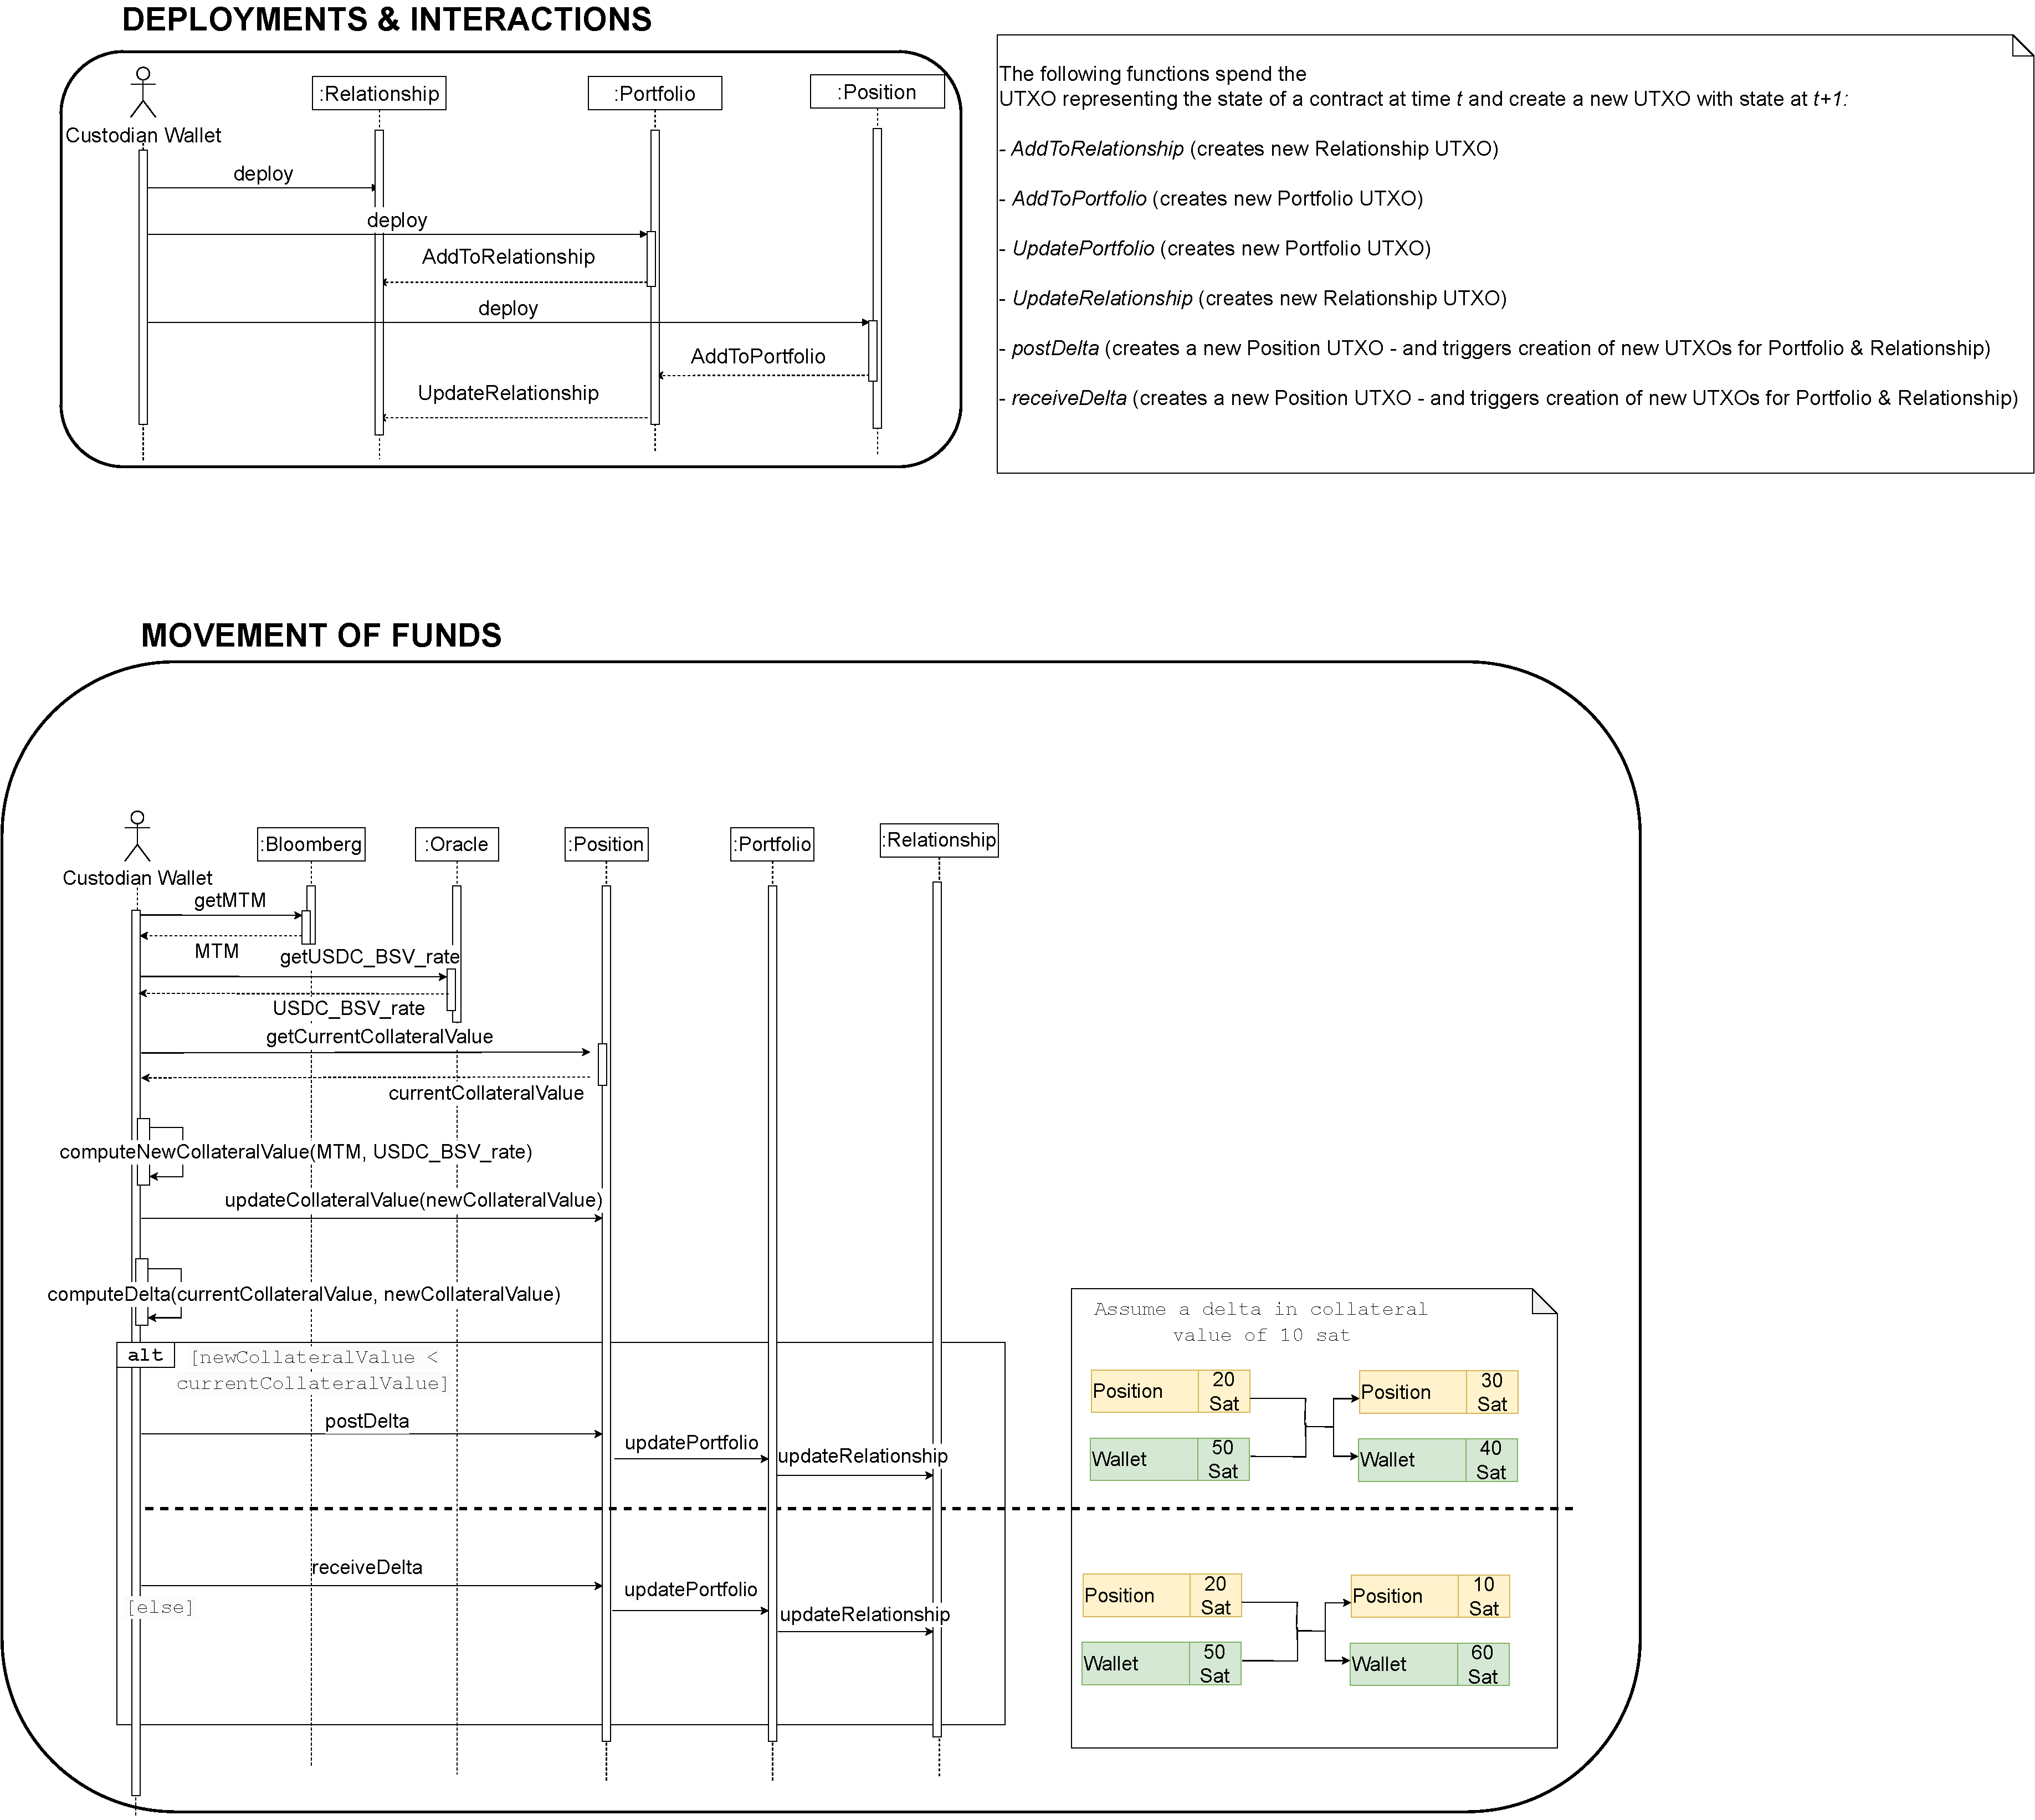
\includegraphics[angle=90, height=\textheight, width=\textwidth]{images/chapter 3/sequenceDiagram.drawio.pdf}
    \caption[Sequence Diagram]{Sequence diagrams depicting the steps in the collateral smart contract lifecycle. The upper diagram displays the initial deployment of three smart contracts: Relationship, Portfolio, and Position. The lower diagram illustrates the process of reassessing collateral value due to market shifts, incorporating data from oracles and financial APIs. It also showcases the adjustment of satoshi amounts to align with collateral valuation changes.}
    \label{fig:sequence-diagram}
\end{figure}
\restoregeometry
